\section{Methods}


\subsection{Project Methodology}
When working in a project it is generally a good idea to work according to a predetermined project methodology model. This tends to make the work more effective and produce better quality. That is, more is produced during the same amount of time, the final product is more thought out, better teamwork etc.

Simply, if you have a plan at the start it is easier to stick to that plan and stay on the same path as intended, rather than shifting to another one. That is not to say that the plan cannot change, but if it does it does so controllably.

A historically good model has been the waterfall model. However, in the software industry this has changed lately with the agile methodology being more popular and has proven to be very effective.

\subsubsection{Agile}
Basically, the agile model says that rather than planning a workload for 6 months forward or so it is better to work in short iterations.


\subsection{Matlab prototype}


\subsection{Tensorflow and Machine Learning}

\subsection{AR implementation in ARKit}

\begin{figure}[hbtp]
\begin{center}
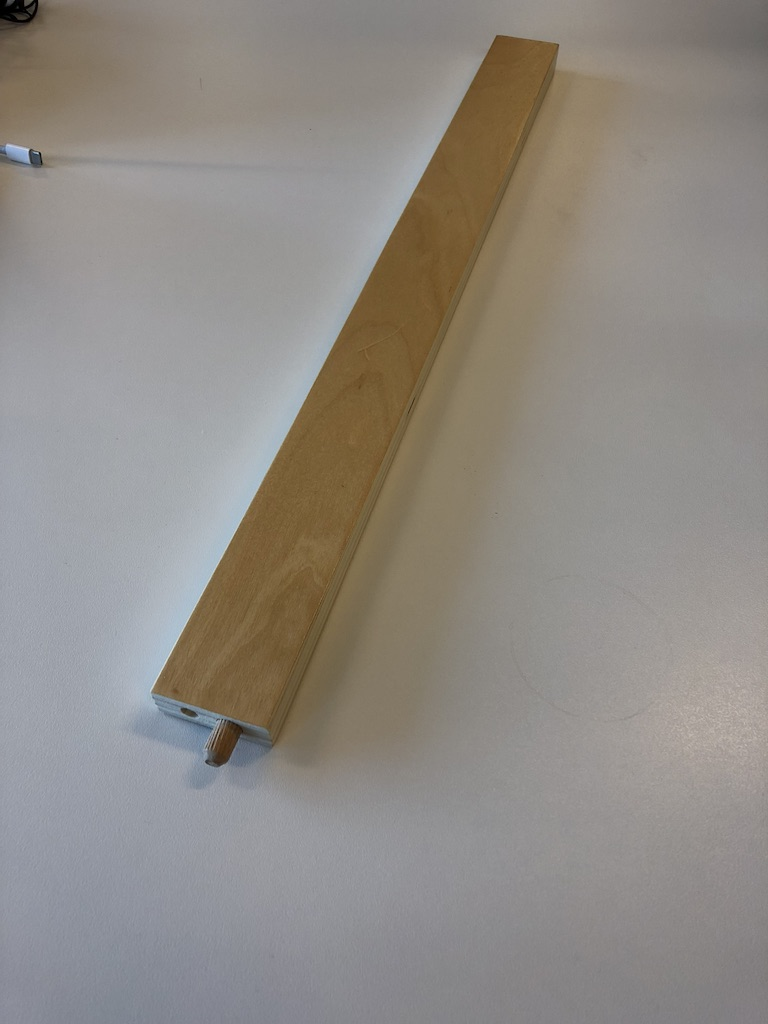
\includegraphics[width = 0.5\textwidth]{./Images/im1.jpg} 
\caption{Example image}
\end{center}
\end{figure}

\newpage